\documentclass[a4paper,12pt]{memoir} % Font and paper size
\usepackage{hyperref} 
%%%%%%%%%%%%%%%%%%%%%%%%%%%%%%%%%%%%%%%%%
% Wenneker Resume/CV
% Structure Specification File
% Version 1.1 (19/6/2016)
%
% This file has been downloaded from:
% http://www.LaTeXTemplates.com
%
% Original author:
% Frits Wenneker (http://www.howtotex.com) with extensive modifications by 
% Vel (vel@latextemplates.com)
%
% License:
% CC BY-NC-SA 3.0 (http://creativecommons.org/licenses/by-nc-sa/3.0/)
%
%%%%%%%%%%%%%%%%%%%%%%%%%%%%%%%%%%%%%%%%%

%----------------------------------------------------------------------------------------
%	PACKAGES AND OTHER DOCUMENT CONFIGURATIONS
%----------------------------------------------------------------------------------------

\usepackage{XCharter} % Use the Bitstream Charter font
\usepackage[utf8]{inputenc} % Required for inputting international characters
\usepackage[T1]{fontenc} % Output font encoding for international characters

\usepackage[top=1cm,left=1cm,right=1cm,bottom=1cm]{geometry} % Modify margins

\usepackage{graphicx} % Required for figures

\usepackage{flowfram} % Required for the multi-column layout

\usepackage{url} % URLs

\usepackage[usenames,dvipsnames]{xcolor} % Required for custom colours

\usepackage{tikz} % Required for the horizontal rule

\usepackage{enumitem} % Required for modifying lists
\setlist{noitemsep,nolistsep} % Remove spacing within and around lists

\setlength{\columnsep}{\baselineskip} % Set the spacing between columns

% Define the left frame (sidebar)
\newflowframe{0.2\textwidth}{\textheight}{0pt}{0pt}[left]
\newlength{\LeftMainSep}
\setlength{\LeftMainSep}{0.2\textwidth}
\addtolength{\LeftMainSep}{1\columnsep}
 
% Small static frame for the vertical line
\newstaticframe{1.5pt}{\textheight}{\LeftMainSep}{0pt}
 
% Content of the static frame with the vertical line
\begin{staticcontents}{1}
\hfill
\tikz{\draw[loosely dotted,color=RoyalBlue,line width=1.5pt,yshift=0](0,0) -- (0,\textheight);}
\hfill\mbox{}
\end{staticcontents}
 
% Define the right frame (main body)
\addtolength{\LeftMainSep}{1.5pt}
\addtolength{\LeftMainSep}{1\columnsep}
\newflowframe{0.7\textwidth}{\textheight}{\LeftMainSep}{0pt}[main01]

\pagestyle{empty} % Disable all page numbering

\setlength{\parindent}{0pt} % Stop paragraph indentation

%----------------------------------------------------------------------------------------
%	NEW COMMANDS
%----------------------------------------------------------------------------------------

\newcommand{\userinformation}[1]{\renewcommand{\userinformation}{#1}} % Define a new command for the CV user's information that goes into the left column

\newcommand{\cvheading}[1]{{\Huge\bfseries\color{RoyalBlue} #1} \par\vspace{.6\baselineskip}} % New command for the CV heading
\newcommand{\cvsubheading}[1]{{\Large\bfseries #1} \bigbreak} % New command for the CV subheading

\newcommand{\Sep}{\vspace{1em}} % New command for the spacing between headings
\newcommand{\SmallSep}{\vspace{0.5em}} % New command for the spacing within headings

\newcommand{\aboutme}[2]{ % New command for the about me section
\textbf{\color{RoyalBlue} #1}~~#2\par\Sep
}
	
\newcommand{\CVSection}[1]{ % New command for the headings within sections
{\Large\textbf{#1}}\par
\SmallSep % Used for spacing
}

\newcommand{\CVItem}[2]{ % New command for the item descriptions
\textbf{\color{RoyalBlue} #1}\par
#2
\SmallSep % Used for spacing
}

\newcommand{\bluebullet}{\textcolor{RoyalBlue}{$\circ$}~~} % New command for the blue bullets


\userinformation{
\begin{flushleft}
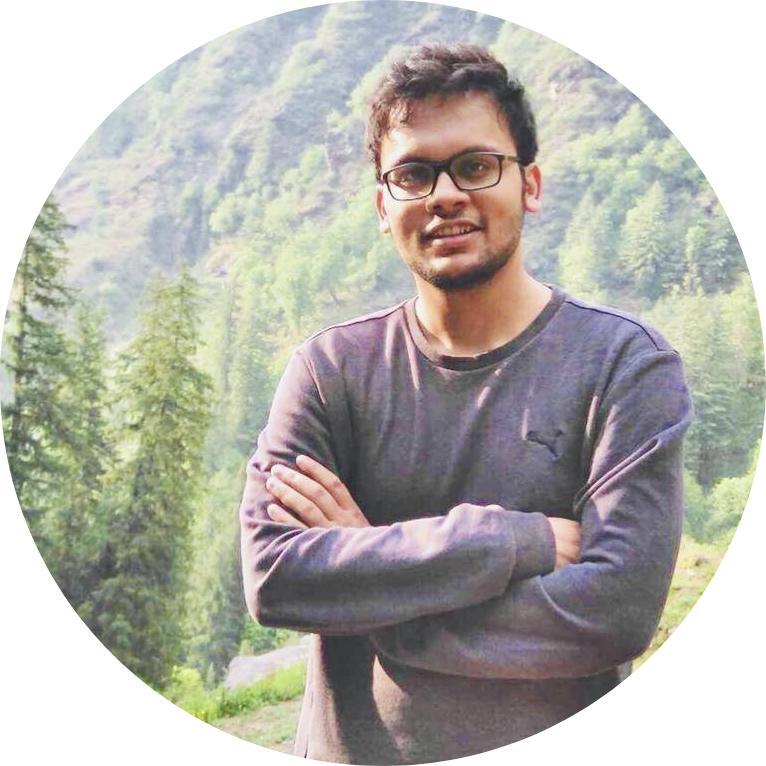
\includegraphics[width=1.0\columnwidth]{photo.png}\\[\baselineskip] % Your photo
\small % Smaller font size
\Sep
\textbf{Website} \\
\href{https://kartikgt.github.io/}{\texttt{kartikgt.github.io}}\\
\Sep
\textbf{Mail} \\
\href{mailto:kartikgt23@gmail.com}{\texttt{kartikgt23@gmail.com}}\\
\Sep
\textbf{Contact} \\
(+91) 9800131277\\
\Sep
\textbf{Programming}\\
\begin{tabular}{p{0.1\textwidth} p{0.1\textwidth}}
\bluebullet Java & \bluebullet Python\\
\bluebullet Shell & \bluebullet SQL\\
\end{tabular}

\Sep
\textbf{Python Libraries}\\
\begin{tabular}{p{0.15\textwidth}}
\bluebullet Requests \\
\bluebullet TensorFlow\\
\bluebullet Keras\\
\bluebullet Beautiful Soup\\
\bluebullet Pandas\\
\bluebullet Matplotlib\\
\bluebullet Selenium\\
\end{tabular}

\Sep
\textbf{Big Data Tools}\\
\begin{tabular}{p{0.1\textwidth} p{0.1\textwidth}}
\bluebullet Hadoop & \bluebullet Hive\\
\bluebullet Grafana & \bluebullet Spark\\
\bluebullet Jenkins  & \bluebullet Splunk\\
\bluebullet MySQL & \bluebullet ELK\\
\end{tabular}

\Sep
\textbf{Operating Systems}\\
\begin{tabular}{p{0.1\textwidth} p{0.1\textwidth}}
\bluebullet Windows & \bluebullet Linux\\
\end{tabular}

\Sep
\textbf{Interests}\\
\begin{tabular}{p{0.17\textwidth}}
\bluebullet Football \\
\bluebullet Formula One\\
\bluebullet Science Fiction\\
\bluebullet History and Arts\\
\bluebullet Swimming\\
\bluebullet Writing blogs\\
\end{tabular}

\vfill % Whitespace under this block to push it up under the photo
\end{flushleft}
}

\begin{document}

\userinformation
\framebreak % End of the first column
\cvheading{Kartik Gupta}

%\cvsubheading{Data Engineer} % Subheading - your occupation/specialization
\CVSection{Education}
\CVItem{2013 - 2018, \textit{Indian Institute of Technology Kharagpur}}{Integrated Dual Degree, Electronics and Electrical Engineering}{
\begin{itemize}
	\item \textbf{Masters' Thesis Project}: Translating Images to Natural Language Sentences using Deep Neural Networks for Captioning.
	\item \textbf{Bachelors' Thesis Project}: Blur kernel estimation in images using a softmax criterion with a Convolutional Neural Network.
\end{itemize}
}
\Sep

\CVSection{Experience}
\CVItem{Jun 2018 - present, \textit{Big Data Engineer}, SAP SuccessFactors}{
\begin{itemize}
	\item Member of the Integrations team of the Cloud Operations Board at SAP Labs, ensuring the operational goals are met and providing seamless integration between cloud based (HCM) applications.
	\item Developed a data democratization platform for developers to manage and monitor their S2 jobs and APIs in real time enabling them to proactively predict and resolve issues before client impact.
	\item Visualized the Application Performance Metrics (APM) in ELK for analyzing page latencies, traffic, and usage trends for applications. 
	\item Created CI/CD paradigm on data pipelines to automate the Extract, Transform, Load (ETL) functions on batch and steaming data.
	\item Applied Machine Learning models to predict job failures, possible downtimes and long running queries, and identified client specific trends for better management of resources during peak season
\end{itemize}
}

\CVItem{May 2017 - Jul 2017, \textit{Operations Intern}, Nomura Research Institute}{
\begin{itemize}
	\item Executed a data governance project for the compliance of a broker back office data ecosystem with the data privacy GDPR guidelines.
	\item Developed solutions for ensuring data integrity, encryption of PIIs, and data mapping by identifying lineages in 50,000+ schemas.
\end{itemize}
}

\CVItem{May 2016 - Jul 2016, \textit{Summer Intern}, Miebach Consulting}{
\begin{itemize}
	\item Identified key Indian ports and industries for introduction of cold storage, CFS and ICDs to support existing supply chain systems.
	\item Formulated an Auto Replenishment System for a retail client to ensure constant stock availability and capacity prediction.
\end{itemize}
}
\Sep

\CVSection{Extra-Curricular}
%\CVItem{Technical}
%{\begin{tabular}{p{0.2\textwidth} p{0.2\textwidth} p{0.2\textwidth}}
%\bluebullet Java &  \bluebullet Shell & \bluebullet Python\\
%\end{tabular}}\\


\CVItem{April 2014 - May 2018, Spring Fest, cultural fest of IIT Kharagpur}{
\begin{itemize}
	\item \textit{Steering Committee Member}, Advised and mentored a team of 50+ students responsible for organizing and conducting the fest.
	\item \textit{Events Head}, Responsible for conceptualizing, planning, and executing the events held during the 59th edition. Led a team of 25+ students and formed partnerships with 10+ associations.
\end{itemize}
}

\CVItem{April 2016, Candidate for the President of the Students' Senate}{
\begin{itemize}
	\item Among the two candidates selected from a batch of 1400+ to contest for the top post in the student body. Presented the Statement of Purpose to 10,000+ students demonstrating public speaking skills. 
	
\end{itemize}
}

\textbf{MISSION} : I aim to develop a full stack Machine Learning Engineering skill-set and apply them to solve complex problems for organizations.

%\Sep % Extra whitespace after the end of a major section
%\clearpage % Start a new page
%\userinformation % Print your information in the left column
%\framebreak % End of the first column
\Sep
\end{document}